\documentclass{article} 
\usepackage{main}
\usepackage[hyphens]{url}  % DO NOT CHANGE THIS
\usepackage{graphicx} % DO NOT CHANGE THIS
\urlstyle{rm} % DO NOT CHANGE THIS
\def\UrlFont{\rm}  % DO NOT CHANGE THIS
%\usepackage{cite}  % DO NOT CHANGE THIS AND DO NOT ADD ANY OPTIONS TO IT
\usepackage{caption} % DO NOT CHANGE THIS AND DO NOT ADD ANY OPTIONS TO IT
\usepackage[utf8]{inputenc} % allow utf-8 input
\usepackage[T1]{fontenc}    % use 8-bit T1 fonts
%\usepackage{hyperref}       % hyperlinks
\usepackage{url}            % simple URL typesetting
\usepackage{booktabs}       % professional-quality tables
\usepackage{amsfonts}       % blackboard math symbols
\usepackage{nicefrac}       % compact symbols for 1/2, etc.
\usepackage{microtype}      % microtypography
\usepackage{xcolor}  % colors
\usepackage{float}
\usepackage{amsmath}
\usepackage[normalem]{ulem}
\usepackage{cancel}
\usepackage{natbib}
\allowdisplaybreaks
\usepackage[none]{hyphenat}
\newtheorem{theorem}{Theorem}[section]
\newtheorem{proposition}[theorem]{Proposition}
\newtheorem{lemma}{Lemma}[section]
\newtheorem{corollary}[theorem]{Corollary}
\newtheorem{definition}[theorem]{Definition}
\newtheorem{assumption}[theorem]{Assumption}
\newtheorem{remark}[theorem]{Remark}
\newtheorem{fact}[theorem]{Fact}
\newtheorem{proof}[theorem]{Proof}

\title{Robust Reinforcement Learning under Environmental Uncertainty and Adversarial Disturbances}
\renewcommand{\undertitle}{Mid-Semester Project Report}

\author{{Ayush Chauhan} \\
	2023B5A71089P\\
    Department of Computer Science
}

\begin{document}

\maketitle

\begin{abstract}
Deep reinforcement learning (RL) policies are typically trained and evaluated within identical, stationary simulation environments assuming noise-free observations, instantaneous actuation, and fixed physical parameters. When deployed in the real world, however, agents encounter sensor noise, adversarial spoofing, actuation latency, and shifted physical dynamics. In this mid-semester study, we investigate the baseline fragility of standard continuous-control RL policies across two MuJoCo locomotion benchmarks with contrasting stability mechanics: \texttt{Walker2d-v5} (an upright bipedal walker vulnerable to falling) and \texttt{HalfCheetah-v5} (a mechanically stable planar runner). We train Soft Actor-Critic (SAC) agents for $300{,}000$ steps across multiple random seeds on clean environments, freeze the learned policies, and systematically stress-test them across five graded disturbance types spanning three channels: sensor inputs (random Gaussian noise and 10-step white-box Projected Gradient Descent adversarial attacks), actuation (control-step action delay), and physical dynamics (body mass scaling and ground friction scaling). For each disturbance, we quantify the degradation onset ($\epsilon_{80}$) and failure breaking point ($\epsilon_{50}$). Our empirical findings reveal that (1) action latency is catastrophic, with a single delayed step reducing return by $31\%$ on \texttt{Walker2d-v5} and $70\%$ on \texttt{HalfCheetah-v5}, and two steps causing total policy collapse; (2) white-box adversarial sensor perturbations are $2.4\times$ to $3.2\times$ more damaging than random Gaussian noise of identical magnitude, inducing twice the policy action deviation; and (3) sensitivity to physical parameter shifts is strongly asymmetric and dictated by robot mechanics. These failure curves establish the diagnostic foundation for our end-semester investigation into cross-perturbation robustness transfer.
\end{abstract}


\section{Introduction and Motivation}

Reinforcement learning (RL) formulates sequential decision-making under uncertainty by optimizing a policy $\pi$ within a Markov Decision Process (MDP) $\mathcal{M}_{\text{train}} = (\mathcal{S}, \mathcal{A}, P_{\text{train}}, R, \gamma)$. In standard empirical practice, the evaluation environment $\mathcal{M}_{\text{test}}$ is identical to $\mathcal{M}_{\text{train}}$. In practical robotic deployment, this assumption is routinely violated: onboard sensors experience thermal noise or malicious spoofing, communication buses introduce actuation delays, payloads alter the robot's mass and inertia, and surface conditions alter contact friction \citep{gu2025robust}.

The overarching research question of this project is:
\begin{quote}
\emph{Can an RL agent continue to perform well when the deployment environment differs from training conditions---including under adversarial disturbances---and which type of distribution shift is most damaging to a trained policy?}
\end{quote}

Before designing or evaluating robust training strategies, it is essential to rigorously characterize \textbf{how, where, and at what intensity standard non-robust RL policies fail}. In this mid-semester phase, we address this diagnostic question through four concrete contributions:
\begin{enumerate}
    \item We train baseline Soft Actor-Critic (SAC) \citep{haarnoja2018soft} agents to strong performance on two continuous-control MuJoCo environments with identical state-action dimensions ($17\text{-D}$ state, $6\text{-D}$ action) but contrasting failure mechanics: \texttt{Walker2d-v5} and \texttt{HalfCheetah-v5}.
    \item We implement a modular perturbation suite injecting five graded disturbances across three MDP interaction channels: random sensor noise, white-box adversarial sensor attacks, actuation delay, body mass scaling, and ground friction scaling.
    \item Using Common Random Numbers (CRN) across $2{,}580$ evaluation episodes, we map normalized degradation curves and compute exact interpolation thresholds for degradation onset ($\epsilon_{80}$, $20\%$ loss) and policy failure ($\epsilon_{50}$, $50\%$ loss).
    \item We analyze the underlying failure mechanisms via bipedal fall rates and policy action sensitivity $\|\pi(\tilde{s}) - \pi(s)\|_2$.
\end{enumerate}


\section{Background and Related Work}

\subsection{Distributionally Robust and Adversarial MDPs}
Classical Robust MDPs replace the fixed transition kernel $P_0$ with an uncertainty set $\mathcal{U}_\rho(P_0)$ and solve the max-min problem $\max_\pi \min_{P \in \mathcal{U}_\rho(P_0)} J(\pi, P)$. While traditional distributionally robust RL (DRRL) algorithms require a generative model to sample arbitrary state-action pairs, \citet{liang2024single} recently introduced \textbf{Distributionally Robust Q-learning (DRQ)}, the first model-free algorithm capable of learning distributionally robust policies from a \emph{single online trajectory} via the dual formulation of $f$-divergence uncertainty sets and multi-timescale stochastic approximation.

\subsection{Robustness Against Data Corruption and Observation Attacks}
When an adversary corrupts training transitions with cumulative budget $C$, standard maximum likelihood estimation (MLE) in model-based RL degrades severely. \citet{ye2024towards} proposed \textbf{CR-OMLE} and \textbf{CR-PMLE}, weighting transition samples by Total Variation (TV)-based information ratios to achieve an optimal additive regret bound $\tilde{\mathcal{O}}(\sqrt{T} + C)$.

On the observation side, \citet{zhang2020robust} formalized the State-Adversarial MDP (SA-MDP), where an attacker perturbs the observed state $\tilde{s} = s + \delta$ within an $\ell_\infty$ ball while leaving the true physical state $s$ unchanged. Recently, \citet{zhou2025robust} demonstrated that adversarial training against a deterministic worst-case attacker causes policies to overfit to that specific attack direction; they proposed \textbf{ATSA}, a maximum-entropy stochastic adversary that generates diverse perturbations to improve generalization.

\subsection{Unified Robust RL Benchmarks}
\citet{gu2025robust} introduced \textbf{Robust Gymnasium}, categorizing disruptions into four modular channels: observation, action, reward, and environment dynamics. Their benchmark evaluation revealed that neither standard RL algorithms (PPO, SAC) nor specialized robust methods maintain resilience across all disruption channels---motivating our systematic investigation into cross-channel fragility and robustness transfer.


\section{Problem Formulation and Disturbance Taxonomy}

Let $\mathcal{M}_{\text{train}} = (\mathcal{S}, \mathcal{A}, P, R, \gamma)$ denote the nominal training MDP, and let $\pi_\theta: \mathcal{S} \to \mathcal{A}$ denote the deterministic evaluation policy (alongside twin critics $Q_{\phi_1}, Q_{\phi_2}: \mathcal{S} \times \mathcal{A} \to \mathbb{R}$) obtained after training on $\mathcal{M}_{\text{train}}$. At test time, the network parameters $(\theta, \phi_1, \phi_2)$ are frozen.

A test-time disturbance is parameterized by a pair $(k, \epsilon)$ representing the disturbance type $k$ and intensity $\epsilon$. As summarized in Table~\ref{tab:taxonomy}, the five disturbances enter the agent--environment loop at three distinct points:

\begin{table}[H]
\centering
\caption{Taxonomy of the five test-time disturbances evaluated in this study.}
\label{tab:taxonomy}
\resizebox{\textwidth}{!}{%
\begin{tabular}{llll}
\toprule
\textbf{Channel} & \textbf{Disturbance Type ($k$)} & \textbf{Mathematical Formulation} & \textbf{Intensity Unit ($\epsilon$)} \\
\midrule
Sensor Input & Random Sensor Noise (\texttt{obs\_noise}) & $\tilde{s}_t = s_t + \epsilon \sigma_s \odot \xi_t, \; \xi_t \sim \mathcal{N}(0, I)$ & $\times$ per-dim state std $\sigma_s$ \\
Sensor Input & Adversarial Attack (\texttt{obs\_adv}) & $\tilde{s}_t = s_t + \arg\min_{|\delta_i| \le \epsilon \sigma_{s,i}} Q(s_t, \pi_\theta(s_t + \delta))$ & $\times$ per-dim state std $\sigma_s$ \\
Actuator & Action Delay (\texttt{act\_delay}) & $\tilde{a}_t = a_{t - \epsilon}$ (FIFO queue of length $\epsilon$) & Control steps ($\mathbb{Z}_{\ge 0}$) \\
Physics & Body Mass Scale (\texttt{mass}) & $m_b \leftarrow \epsilon m_b, \; I_b \leftarrow \epsilon I_b \; (\forall \text{ bodies } b)$ & Multiplier ($\epsilon = 1.0$ nominal) \\
Physics & Ground Friction Scale (\texttt{friction}) & $\mu_{\text{slide}} \leftarrow \epsilon \mu_{\text{slide}} \; (\forall \text{ geoms})$ & Multiplier ($\epsilon = 1.0$ nominal) \\
\bottomrule
\end{tabular}%
}
\end{table}

\paragraph{Theoretical Distinction Between Channels.}
Sensor perturbations (\texttt{obs\_noise} and \texttt{obs\_adv}) do \emph{not} alter the underlying physical transition kernel $P(s_{t+1} \mid s_t, a_t)$; rather, they corrupt the policy input $a_t = \pi_\theta(\tilde{s}_t)$. Conversely, actuation delay (\texttt{act\_delay}) violates the first-order Markov assumption by coupling the transition to past actions $a_{t-\epsilon}$, while physical perturbations (\texttt{mass} and \texttt{friction}) directly modify the rigid-body dynamics $P_{\text{test}} \neq P_{\text{train}}$. Note that reward corruption is excluded from test-time evaluation because a frozen policy $\pi_\theta(s)$ does not observe rewards during deployment; reward poisoning strictly affects training-time Bellman updates.

\paragraph{White-Box Critic PGD Attack.}
Because state dimensions (joint angles in radians vs.\ angular velocities in rad/s) have heterogeneous scales, we first compute the empirical per-dimension standard deviation $\sigma_s \in \mathbb{R}^{17}$ across $5$ clean trajectories of the trained policy. For the adversarial sensor attack (\texttt{obs\_adv}) with budget $\epsilon$, we solve the constrained minimization:
\begin{equation}
    \delta_t^* = \arg\min_{\|\delta \oslash \sigma_s\|_\infty \le \epsilon} \min_{j \in \{1,2\}} Q_{\phi_j}\big(s_t, \, \pi_\theta(s_t + \delta)\big),
\end{equation}
using $K=10$ iterations of Projected Gradient Descent (PGD) initialized uniformly inside the $\ell_\infty$ box $[-\epsilon \sigma_s, +\epsilon \sigma_s]$ with step size $\alpha = 0.25 \epsilon \sigma_s$:
\begin{equation}
    \delta^{(m+1)} = \Pi_{[-\epsilon \sigma_s, \epsilon \sigma_s]} \left( \delta^{(m)} - \alpha \cdot \text{sign}\big( \nabla_{\delta} \min_{j=1,2} Q_{\phi_j}(s_t, \pi_\theta(s_t + \delta^{(m)})) \big) \right).
\end{equation}
Critically, the critic $Q_{\phi_j}(s_t, \cdot)$ is evaluated at the \emph{true} state $s_t$ and the corrupted action $\pi_\theta(s_t + \delta)$, finding the sensor perturbation that forces the actor to choose the worst possible action for the current physical state \citep{zhang2020robust}.

\paragraph{Evaluation Metrics.}
Let $J(\pi_\theta; k, \epsilon) = \mathbb{E}[\sum_{t=0}^{T} r_t]$ denote the mean empirical episode return of agent $\pi_\theta$ under disturbance $(k, \epsilon)$, and let $J_0 = J(\pi_\theta; \text{clean})$ denote its nominal clean return. We define:
\begin{itemize}
    \item \textbf{Normalized Return:} $\bar{J}(k, \epsilon) = J(\pi_\theta; k, \epsilon) / J_0$, where $\bar{J} = 1.0$ indicates zero degradation.
    \item \textbf{Degradation Onset ($\epsilon_{80}$) and Breaking Point ($\epsilon_{50}$):} The smallest perturbation magnitude moving away from the nominal value at which $\bar{J}(k, \epsilon)$ drops below $0.80$ ($20\%$ performance loss) and $0.50$ ($50\%$ performance loss), respectively, computed via linear interpolation.
    \item \textbf{Fall Rate and Policy Sensitivity:} The fraction of episodes terminating early due to torso collapse (\texttt{Walker2d-v5}), and the mean $\ell_2$ action shift $\|\pi_\theta(\tilde{s}_t) - \pi_\theta(s_t)\|_2$ induced by sensor perturbations.
\end{itemize}


\section{Experimental Setup}

\paragraph{Environments.}
We evaluate two MuJoCo locomotion environments from Gymnasium v1.x \citep{raffin2021stable}, both featuring $\mathcal{S} \subset \mathbb{R}^{17}$ and $\mathcal{A} = [-1, 1]^6$:
\begin{enumerate}
    \item \texttt{Walker2d-v5}: A planar bipedal robot with $6$ actuated joints (left/right hip, knee, ankle). It requires active upright balance; an episode terminates early (a \emph{fall}) if the torso height drops outside $[0.8, 2.0]\text{ m}$ or torso pitch exceeds $\pm 1.0\text{ rad}$. Control step $\Delta t = 8\text{ ms}$.
    \item \texttt{HalfCheetah-v5}: A planar quadruped runner with $6$ actuated joints. It is mechanically prevented from falling and always runs for the full horizon of $H = 1{,}000$ steps. Control step $\Delta t = 50\text{ ms}$.
\end{enumerate}

\paragraph{SAC Training Configuration.}
We train Soft Actor-Critic (SAC) agents using Stable-Baselines3 across $3$ independent random seeds ($0, 1, 2$) per environment for $300{,}000$ environment steps. Why SAC over tabular TD or Monte Carlo methods? Because $\mathcal{S} \subset \mathbb{R}^{17}$ and $\mathcal{A} = [-1, 1]^6$ are continuous, tabular storage is impossible and exact greedy maximization $\arg\max_{a \in \mathcal{A}} Q(s,a)$ cannot be enumerated. Moreover, Monte Carlo estimation suffers from high variance across $1{,}000$-step horizons and cannot reuse off-policy data. SAC overcomes both limitations by combining $1$-step off-policy TD learning on a replay buffer of size $10^6$ (via twin MLP critics of size $256 \times 256$, $\gamma=0.99$, Polyak $\tau=0.005$, batch size $256$, Adam learning rate $3 \times 10^{-4}$) with a continuous actor network $\pi_\theta(s)$ regularized by automatic maximum-entropy exploration.

\paragraph{Stress-Test Protocol.}
Each trained checkpoint is evaluated deterministically across $43$ (disturbance, intensity) conditions for $10$ episodes per condition ($2{,}580$ episodes total). Every condition uses identical environment reset seeds $\{0, 1, \dots, 9\}$ (Common Random Numbers), ensuring that performance differences are attributable solely to the injected disturbance.


\section{Results and Analysis}

\subsection{Clean Baseline Training Performance}

Figure~\ref{fig:learning} displays the clean evaluation learning curves over $300{,}000$ environment steps, and Table~\ref{tab:clean} summarizes the final baseline scores. Both environments converge smoothly with low inter-seed variance. \texttt{HalfCheetah-v5} achieves a clean return of $8245.5 \pm 765.0$, while \texttt{Walker2d-v5} achieves $3788.3 \pm 287.6$ with a low baseline fall rate of $6.7\%$.

\begin{figure}[H]
    \centering
    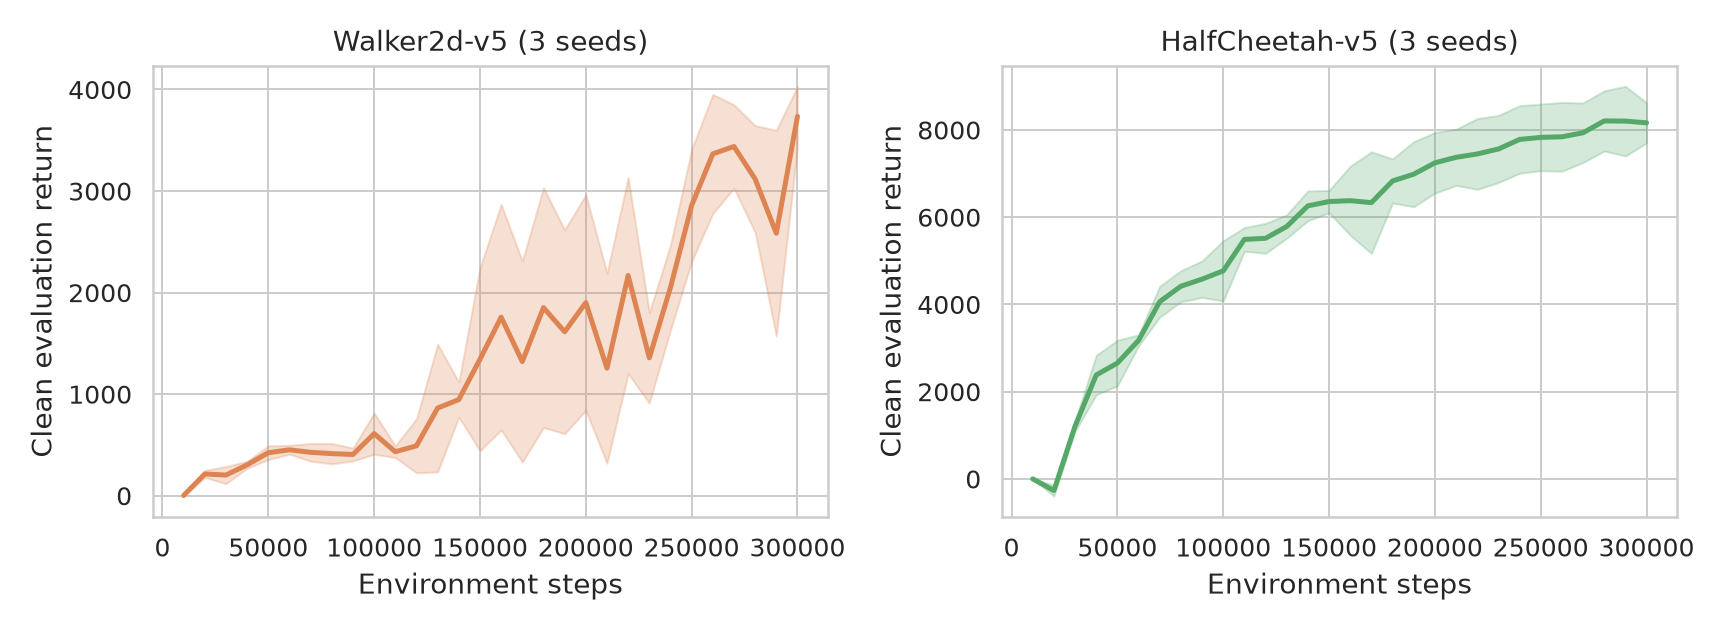
\includegraphics[width=0.88\textwidth]{../figures/learning_curves.png}
    \caption{Clean evaluation return during SAC training across $300{,}000$ environment steps (mean $\pm$ std across $3$ seeds; evaluated every $10{,}000$ steps over $5$ episodes).}
    \label{fig:learning}
\end{figure}

\begin{table}[H]
\centering
\caption{Clean baseline performance of trained SAC agents after $300{,}000$ steps ($3$ seeds $\times$ $10$ evaluation episodes).}
\label{tab:clean}
\begin{tabular}{lccc}
\toprule
\textbf{Environment} & \textbf{Clean Return (Mean $\pm$ Std)} & \textbf{Mean Episode Length} & \textbf{Clean Fall Rate} \\
\midrule
\texttt{HalfCheetah-v5} & $8245.5 \pm 765.0$ & $1000.0$ & $0.0\%$ (cannot fall) \\
\texttt{Walker2d-v5}    & $3788.3 \pm 287.6$ & $980.2$  & $6.7\%$ \\
\bottomrule
\end{tabular}
\end{table}

\subsection{Degradation Curves and Breaking Points Across the 5 Disturbances}

Figures~\ref{fig:degradation} and \ref{fig:absolute} present the normalized and absolute return degradation curves across all five disturbances, while Table~\ref{tab:breaking} reports the exact degradation onset ($\epsilon_{80}$) and failure breaking points ($\epsilon_{50}$). Figure~\ref{fig:heatmap} summarizes retained performance at pre-declared moderate disturbance levels.

\begin{figure}[H]
    \centering
    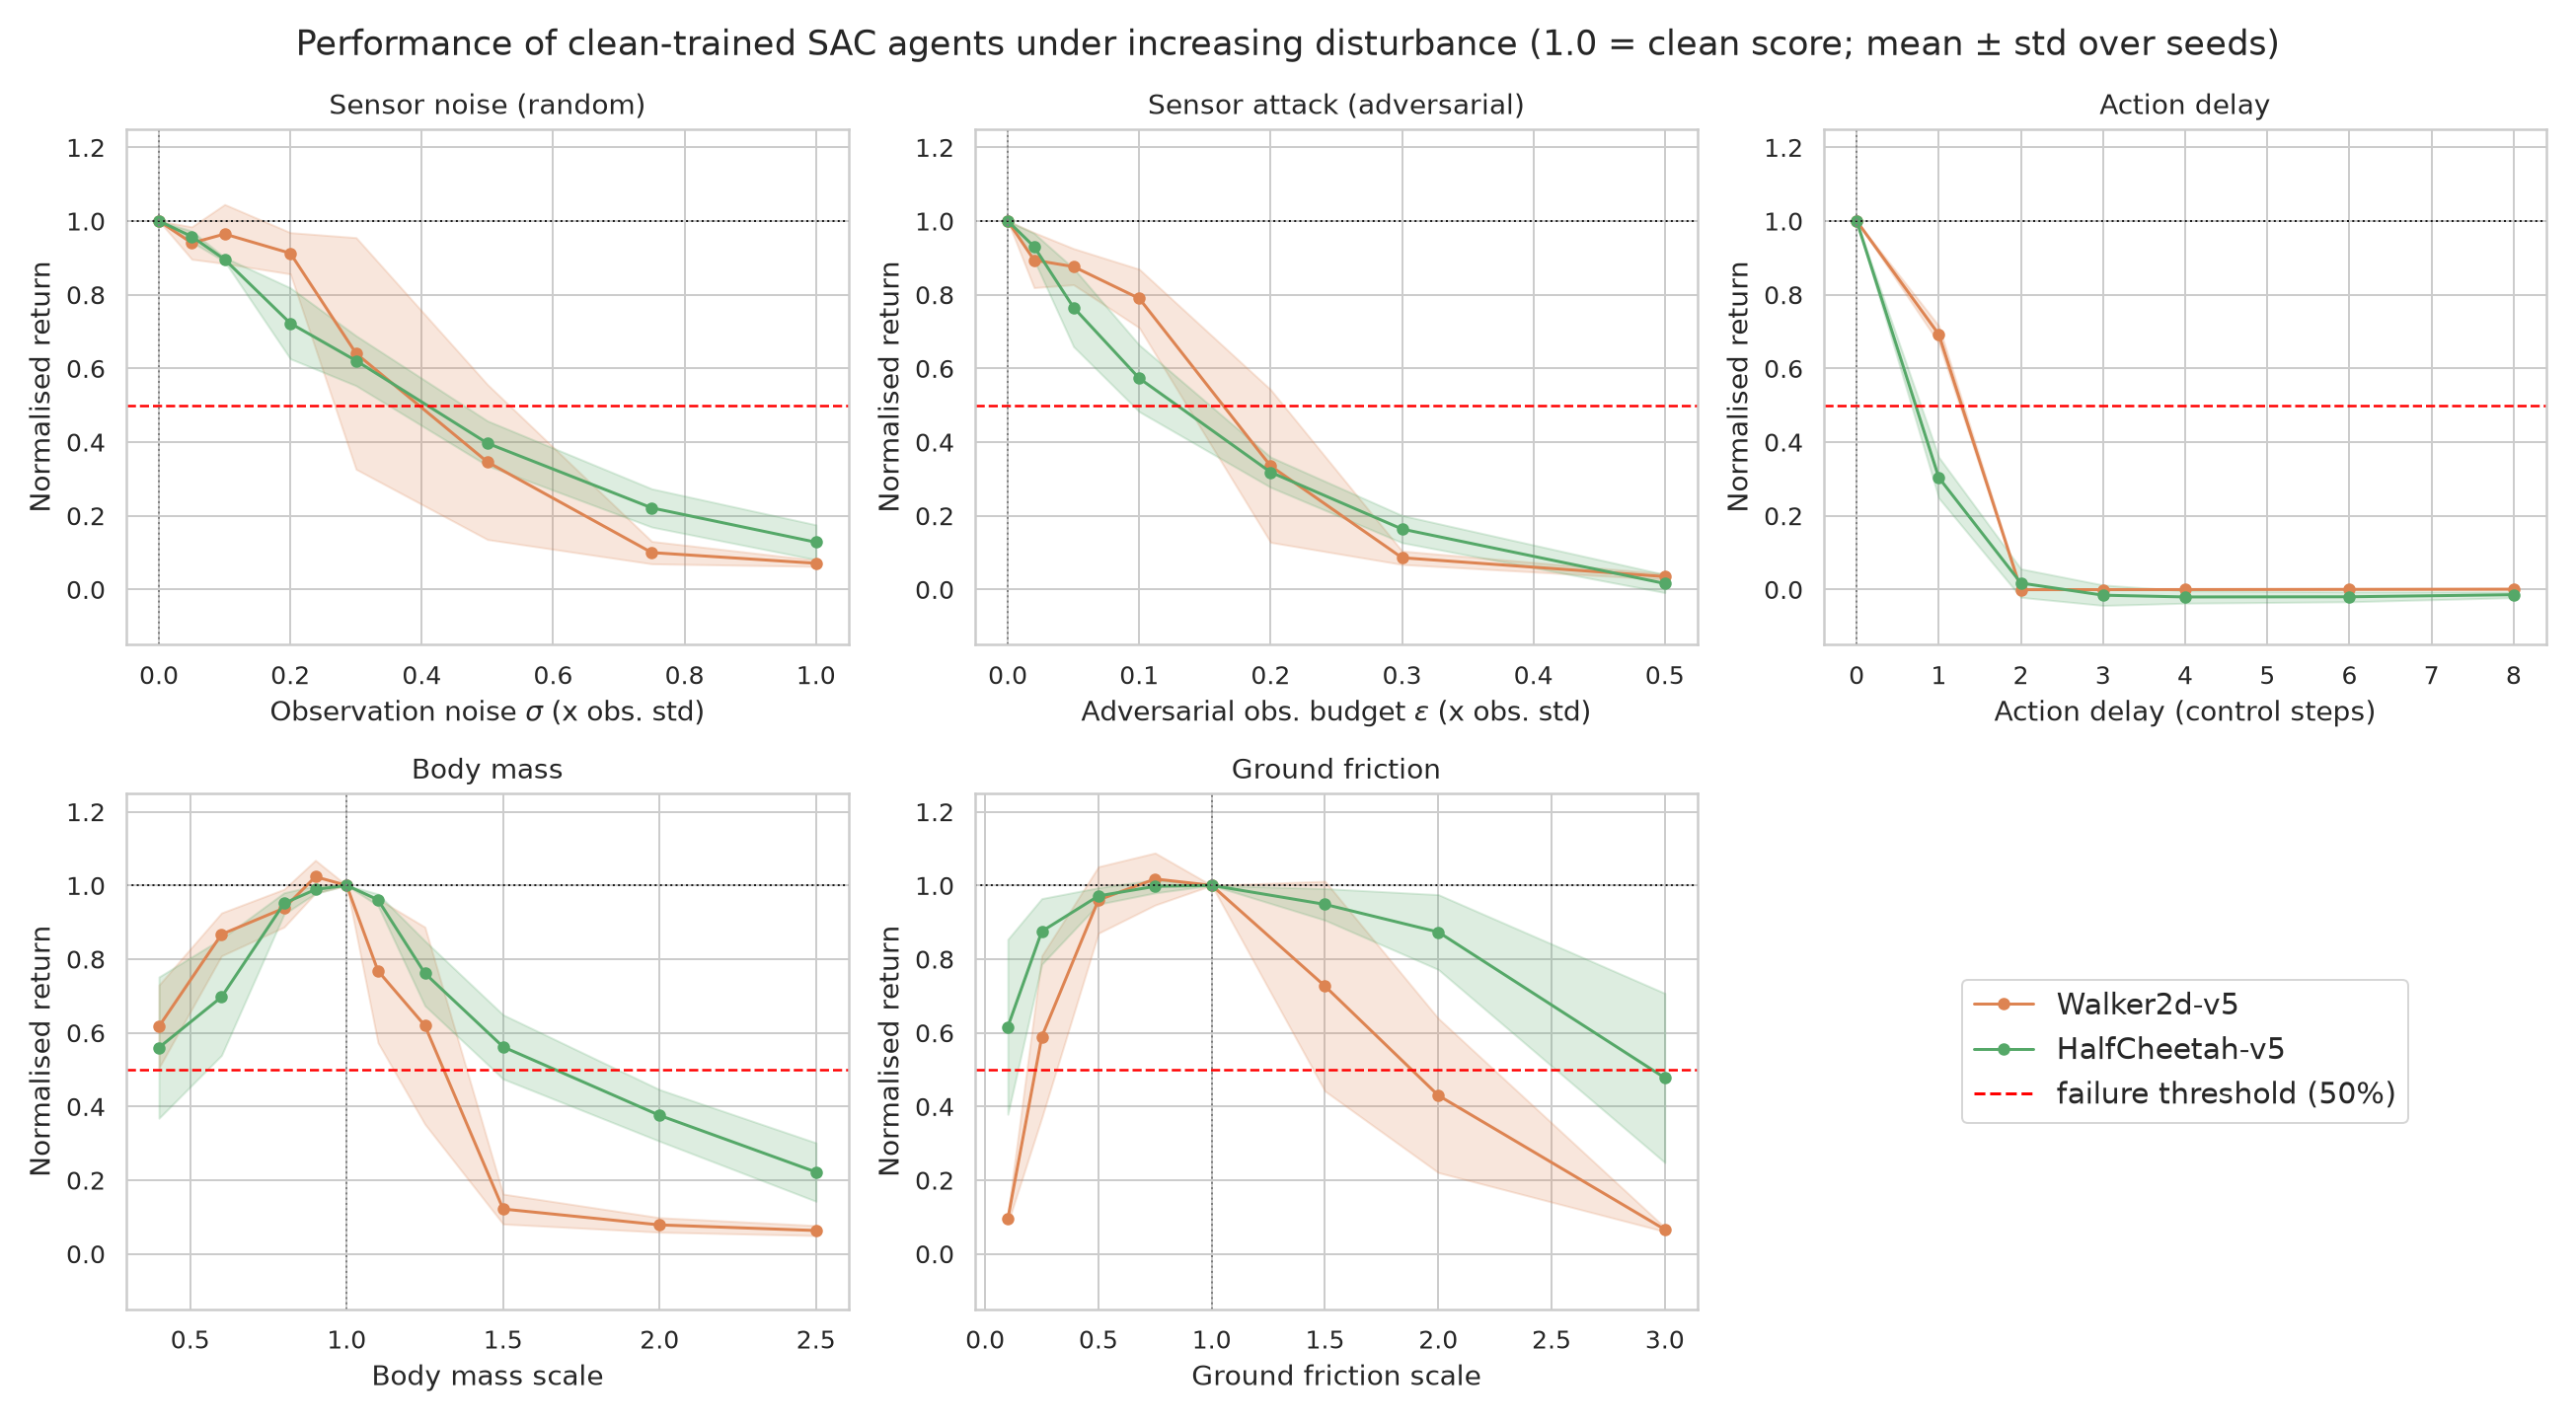
\includegraphics[width=0.98\textwidth]{../figures/degradation_all.png}
    \caption{Normalized return ($\bar{J} = J_{\text{pert}} / J_{\text{clean}}$) of clean-trained SAC agents under increasing disturbance intensity across all five perturbation types (mean $\pm$ std over $3$ seeds). The dashed red line marks the $50\%$ failure threshold ($\epsilon_{50}$).}
    \label{fig:degradation}
\end{figure}

\begin{figure}[H]
    \centering
    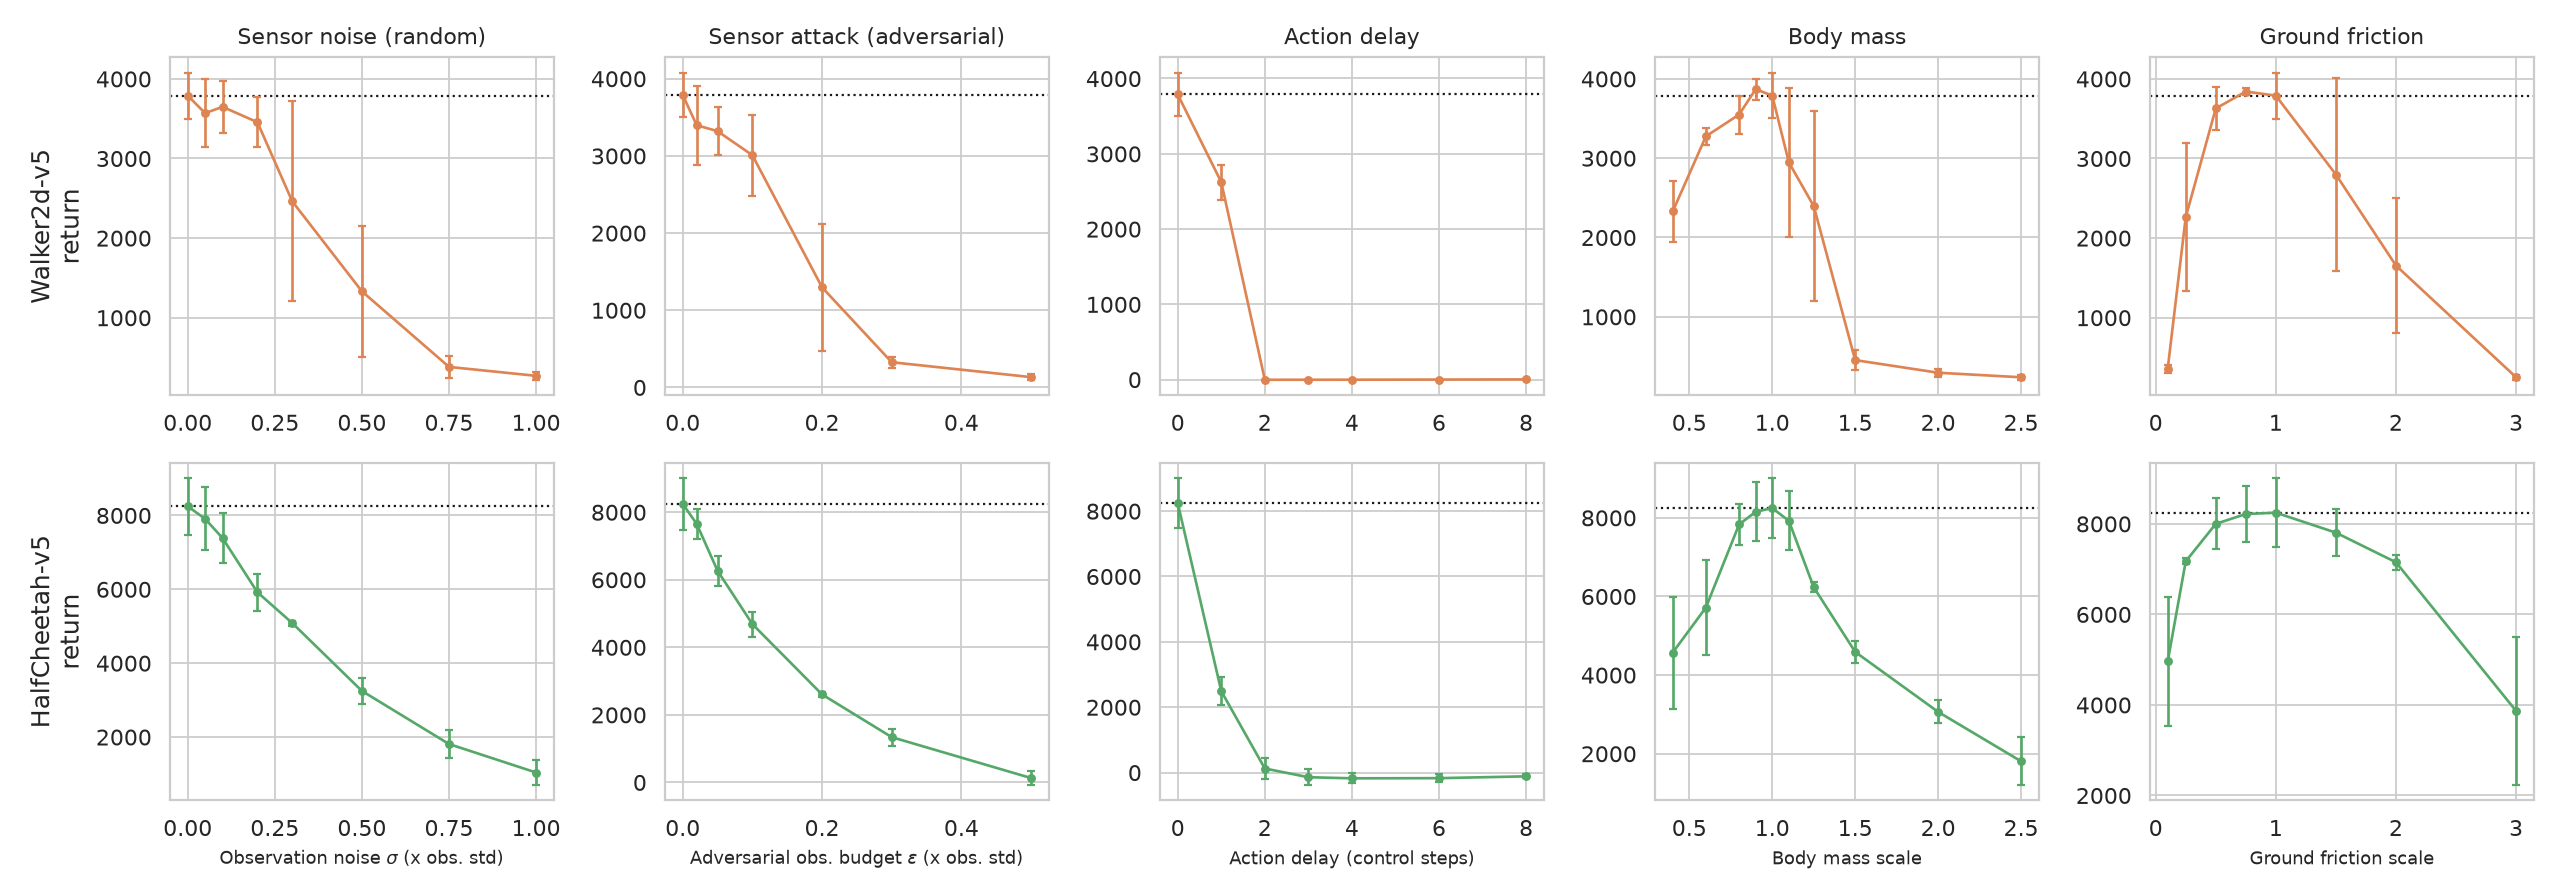
\includegraphics[width=0.98\textwidth]{../figures/degradation_absolute.png}
    \caption{Absolute episode return versus disturbance intensity for \texttt{Walker2d-v5} (top row) and \texttt{HalfCheetah-v5} (bottom row). Dotted black lines indicate nominal clean baseline scores.}
    \label{fig:absolute}
\end{figure}

\begin{table}[H]
\centering
\caption{Degradation onset ($\epsilon_{80}$, where $\bar{J} < 0.80$), failure breaking point ($\epsilon_{50}$, where $\bar{J} < 0.50$), and worst normalized return across all five disturbances (``$\infty$'' indicates threshold not crossed within tested range).}
\label{tab:breaking}
\resizebox{\textwidth}{!}{%
\begin{tabular}{llccc}
\toprule
\textbf{Disturbance Type} & \textbf{Direction / Unit} & \textbf{\texttt{Walker2d-v5} ($\epsilon_{80} / \epsilon_{50}$)} & \textbf{\texttt{HalfCheetah-v5} ($\epsilon_{80} / \epsilon_{50}$)} & \textbf{Worst $\bar{J}$ (Walk / HC)} \\
\midrule
Sensor Noise (\texttt{obs\_noise})  & $\sigma$ ($\times \sigma_s$) & $0.241 \; / \; 0.395$ & $0.155 \; / \; 0.408$ & $0.071 \; / \; 0.128$ \\
Sensor Attack (\texttt{obs\_adv})   & $\epsilon$ ($\times \sigma_s$) & $0.094 \; / \; 0.164$ & $0.044 \; / \; 0.129$ & $0.035 \; / \; 0.016$ \\
Action Delay (\texttt{act\_delay})  & Control steps & $0.649 \; / \; 1.280$ & $0.287 \; / \; 0.718$ & $0.000 \; / \; -0.021$ \\
Body Mass (\texttt{mass})           & Heavier ($\uparrow$) & $\times 1.09 \; / \; \times 1.31$ & $\times 1.22 \; / \; \times 1.67$ & $0.063 \; / \; 0.222$ \\
Body Mass (\texttt{mass})           & Lighter ($\downarrow$) & $\times 0.55 \; / \; \infty$ & $\times 0.68 \; / \; \infty$ & $0.617 \; / \; 0.560$ \\
Ground Friction (\texttt{friction}) & Slippery ($\downarrow$) & $\times 0.39 \; / \; \times 0.22$ & $\times 0.21 \; / \; \infty$ & $0.094 \; / \; 0.616$ \\
Ground Friction (\texttt{friction}) & Sticky ($\uparrow$) & $\times 1.37 \; / \; \times 1.88$ & $\times 2.19 \; / \; \times 2.94$ & $0.066 \; / \; 0.477$ \\
\bottomrule
\end{tabular}%
}
\end{table}

\begin{figure}[H]
    \centering
    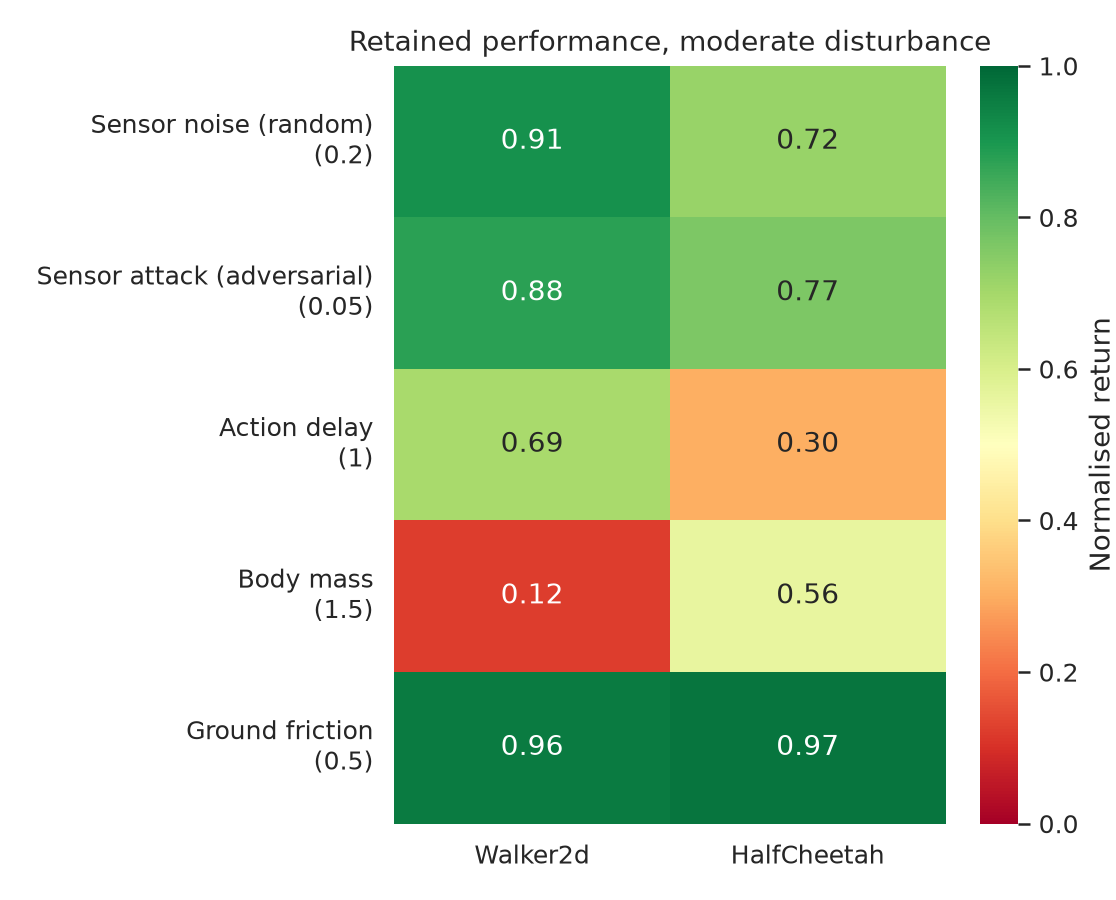
\includegraphics[width=0.58\textwidth]{../figures/heatmap_moderate.png}
    \caption{Retained normalized return under moderate disturbance intensities across both environments.}
    \label{fig:heatmap}
\end{figure}

\subsection{Random Sensor Noise vs.\ Adversarial Sensor Attack}

Figure~\ref{fig:rand_vs_adv} directly compares random Gaussian sensor noise (\texttt{obs\_noise}) against the 10-step PGD critic attack (\texttt{obs\_adv}) on a shared logarithmic perturbation axis. Across both tasks, adversarial perturbations break the policy at \textbf{$2.4\times$ to $3.2\times$ smaller budgets}: on \texttt{Walker2d-v5}, $\epsilon_{50}$ drops from $0.395$ to $0.164$, while on \texttt{HalfCheetah-v5}, $\epsilon_{50}$ drops from $0.408$ to $0.129$. Notably, an adversarial sensor perturbation of just $4.4\%$ of the standard deviation on \texttt{HalfCheetah-v5} reduces total return by $20\%$.

\begin{figure}[H]
    \centering
    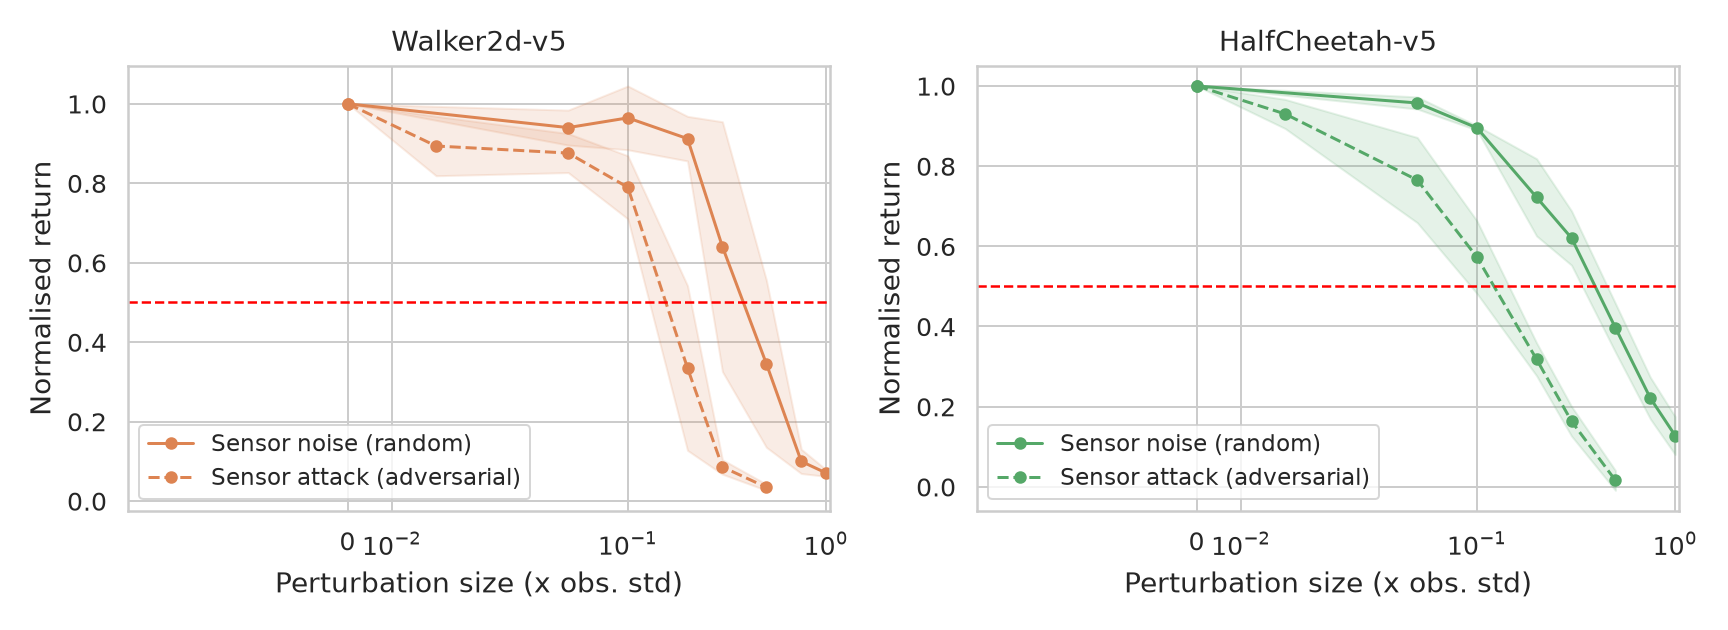
\includegraphics[width=0.88\textwidth]{../figures/random_vs_adversarial.png}
    \caption{Comparison of random Gaussian sensor noise and white-box PGD adversarial sensor attacks at matched per-dimension budgets.}
    \label{fig:rand_vs_adv}
\end{figure}

\subsection{Failure Mechanisms: Bipedal Falls and Policy Sensitivity}

Figure~\ref{fig:falls} illuminates \emph{why} the policies fail:
\begin{enumerate}
    \item \textbf{Abrupt Bipedal Collapse:} On \texttt{Walker2d-v5} (left and middle panels), performance degradation is driven by sudden torso falls. Under adversarial sensor attacks at $\epsilon=0.2$, the fall rate jumps from $6.7\%$ to $90\%$; under a $2$-step action delay, the fall rate reaches $100\%$.
    \item \textbf{Directional Sensitivity of Neural Policies:} The right panel plots the mean action deviation $\|\pi_\theta(\tilde{s}) - \pi_\theta(s)\|_2$. Under random Gaussian noise, action deviation grows linearly with slope $\approx 1.9$ (reflecting the average local Lipschitz constant of the actor MLP). Under PGD attack, the action deviation is \textbf{nearly twice as large} at every budget $\epsilon$, confirming that PGD discovers steep gradient directions of the policy and critic networks.
\end{enumerate}

\begin{figure}[H]
    \centering
    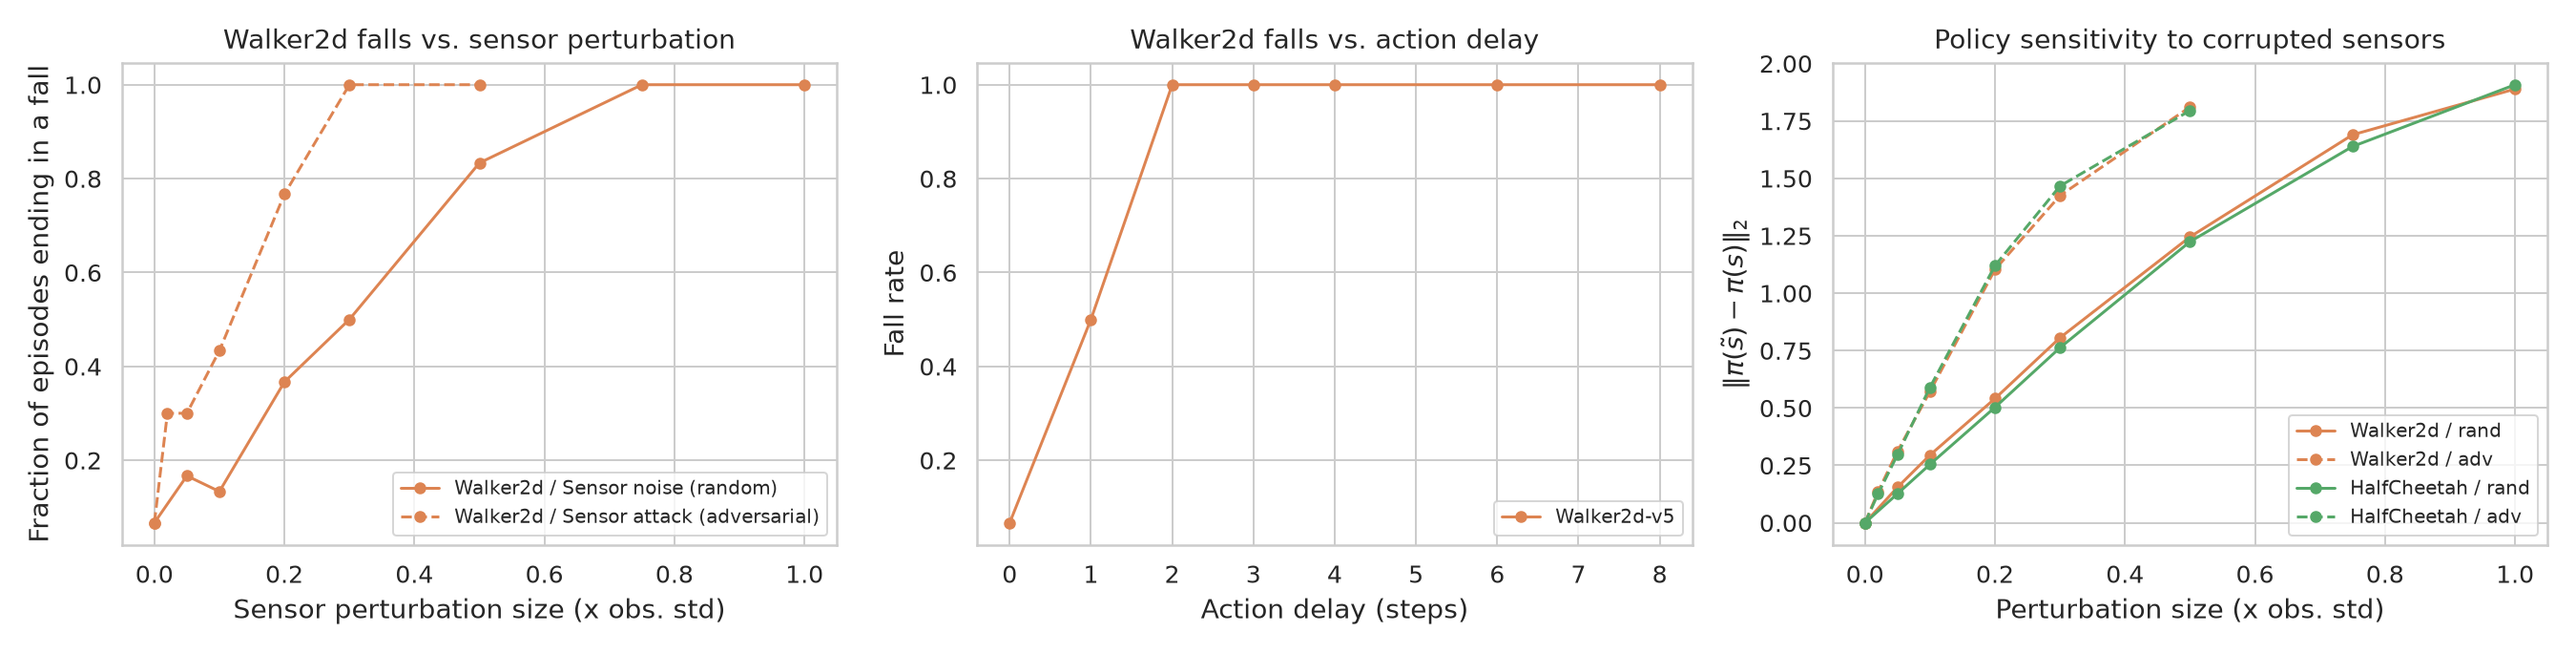
\includegraphics[width=0.98\textwidth]{../figures/falls_and_sensitivity.png}
    \caption{Left: \texttt{Walker2d-v5} fall rate under random vs.\ adversarial sensor perturbations. Middle: \texttt{Walker2d-v5} fall rate vs.\ action delay. Right: Policy action sensitivity $\|\pi_\theta(\tilde{s}) - \pi_\theta(s)\|_2$.}
    \label{fig:falls}
\end{figure}


\section{Discussion of Key Findings}

\paragraph{1. Why is Action Delay the Most Destructive Disturbance?}
A single control step of latency reduces return by $31\%$ on \texttt{Walker2d-v5} and $70\%$ on \texttt{HalfCheetah-v5}, and $2$ steps completely destroys both policies ($\bar{J} \le 0$). Two factors explain this: first, standard MLP policies $\pi_\theta(s_t)$ are memoryless and assume the environment is strictly Markovian; when $a_{t-k}$ is executed instead of $a_t$, the true system state includes the queue of $k$ pending actions, rendering the MDP partially observable. Second, \texttt{HalfCheetah-v5} uses a control timestep of $\Delta t = 50\text{ ms}$ (frame-skip $5 \times 10\text{ ms}$), whereas \texttt{Walker2d-v5} uses $\Delta t = 8\text{ ms}$. Thus, a $1$-step delay corresponds to $50\text{ ms}$ of physical lag in \texttt{HalfCheetah-v5}---over $6\times$ longer in wall-clock physics time than in \texttt{Walker2d-v5}.

\paragraph{2. Why Are Physical Mass Shifts Asymmetric?}
Both agents tolerate lighter body masses well (retaining $>56\%$ return even at $0.4\times$ mass, never crossing $\epsilon_{50}$), but fail rapidly when mass increases ($\epsilon_{50} = 1.31\times$ for \texttt{Walker2d-v5} and $1.67\times$ for \texttt{HalfCheetah-v5}). Because SAC policies maximize forward velocity, they operate near actuator torque saturation limits $[-1, 1]^6$. Increasing body mass increases gravitational load $g(q)$ and inertial resistance $M(q)\ddot{q}$ beyond the maximum torque authority of the motors.

\paragraph{3. Robot Mechanics Dictate Which Physics Shift Hurts Most.}
On slippery surfaces ($0.22\times$ friction), \texttt{Walker2d-v5} loses $50\%$ of its return because foot slippage immediately causes its center of mass to exit its narrow bipedal support polygon, resulting in a fall. In contrast, \texttt{HalfCheetah-v5} cannot fall over and retains $61.6\%$ of its clean score even on near-frictionless ice ($0.1\times$ friction). Consequently, there is no universal ``most damaging'' physical parameter across tasks.


\section{Limitations and End-Semester Roadmap}

\paragraph{Limitations of Current Study.}
First, our evaluation applies disturbances strictly at \emph{test time} across $3$ seeds per environment; training-time reward corruption requires retraining agents under poisoned reward signals and will be conducted in the second phase. Second, because perturbation units differ across channels ($\sigma_s$ multiples vs.\ delay steps vs.\ mass multipliers), raw breaking points cannot be compared across channels without magnitude calibration.

\paragraph{Plan for End-Semester Phase.}
In the second half of the semester, we will transition from \emph{diagnosis} to \emph{defense and transfer}:
\begin{enumerate}
    \item \textbf{Implement Robust Training Strategies:} Observation-noise augmentation, policy smoothness/Lipschitz regularization \citep{zhang2020robust}, domain randomization over mass and friction, distributionally robust pessimistic Q-backups \citep{liang2024single}, and uncertainty-weighted TD losses against reward corruption \citep{ye2024towards}.
    \item \textbf{Cross-Robustness Transfer Matrix:} Systematically train an agent using a defense designed for channel $k$ and evaluate it under channel $k' \neq k$ at performance-calibrated intensities to test whether robustness transfers across perturbation families.
    \item \textbf{Unified Multi-Channel Stochastic Adversary:} Inspired by ATSA \citep{zhou2025robust}, we will design a maximum-entropy adversary that stochastically perturbs observations, actions, and dynamics during training, accompanied by ablation studies.
\end{enumerate}

\bibliography{references}
\bibliographystyle{apalike}

\end{document}
